\documentclass[red]{beamer}
% Class options include: notes, notesonly, handout, trans,
%                        hidesubsections, shadesubsections,
%                        inrow, blue, red, grey, brown


% Theme for beamer presentation.
\usepackage{beamerthemetree} 
% Other themes include: beamerthemebars, beamerthemelined, 
%                       beamerthemetree, beamerthemetreebars  
\usepackage{listings}

\title{D3: Diving into the library}    
\author{David Leonard}                 
\institute{City College of New York}      
\date{\today}                   

\begin{document}

\lstdefinelanguage{JavaScript}{
  keywords={typeof, new, true, false, catch, function, return, null, catch, switch, var, if, in, while, do, else, case, break, this},
  keywordstyle=\color{blue}\bfseries,
  ndkeywords={class, export, boolean, throw, implements, import, this},
  ndkeywordstyle=\color{darkgray}\bfseries,
  identifierstyle=\color{black},
  sensitive=false,
  comment=[l]{//},
  morecomment=[s]{/*}{*/},
  commentstyle=\color{purple}\ttfamily,
  stringstyle=\color{red}\ttfamily,
  morestring=[b]',
  morestring=[b]"
}

\lstset{
   language=JavaScript,
   extendedchars=true,
   basicstyle=\scriptsize\ttfamily,
   showstringspaces=false,
   showspaces=false,
   tabsize=2,
   breaklines=true,
   showtabs=false,
   captionpos=b
}

% Object code listing
\defverbatim[colored]\lstl{
	\begin{lstlisting}
	   var dataset = [ 100, 200, 300, 400, 500 ]; 
	\end{lstlisting}
}

\defverbatim[colored]\lstll{
    \begin{lstlisting}
      var scale = d3.scale.linear()
                    .domain([100, 500])
                    .range([10, 350]);

      scale(100); // Returns 10
      scale(300); // Returns 180
      scale(500); // Returns 350
    \end{lstlisting}
}

\defverbatim[colored]\lstrect{
    \begin{lstlisting}
      <rect x="0" y="0" width="500" height="50"/>
    \end{lstlisting}
}

\defverbatim[colored]\lstcircle{
    \begin{lstlisting}
      <circle cx="250" cy="25" r="25"/>
    \end{lstlisting}
}

\defverbatim[colored]\lstellipse{
    \begin{lstlisting}
      <ellipse cx="250" cy="25" rx="100" ry="25"/>
    \end{lstlisting}
}

\defverbatim[colored]\lstellipse{
    \begin{lstlisting}
      <ellipse cx="250" cy="25" rx="100" ry="25"/>
    \end{lstlisting}
}

\defverbatim[colored]\lstline{
    \begin{lstlisting}
      <line x1="0" y1="0" x2="500" y2="50" stroke="black"/>
    \end{lstlisting}
}

\defverbatim[colored]\lstaxis{
    \begin{lstlisting}
    var xAxis = d3.svg.axis()
                    .scale(xScale)
                    .orient("bottom")
                    .ticks(5);

    var yAxis = d3.svg.axis()
                    .scale(yScale)
                    .orient("left")
                    .ticks(5);
    \end{lstlisting}
}

\defverbatim[colored]\lstcreateaxis{
    \begin{lstlisting}
    svg.append("g")
        .attr("class", "axis")
        .attr("transform", "translate(0," + (h - padding) + ")")
        .call(xAxis);

    svg.append("g")
        .attr("class", "axis")
        .attr("transform", "translate(" + padding + ",0)")
        .call(yAxis);
    \end{lstlisting}
}

\defverbatim[colored]\lstsvgtriangle{
    \begin{lstlisting}
    <svg width="100" height="100">
      <path d=" M 10 25
                L 10 75
                L 60 75
                L 10 25"
                stroke="red" stroke-width="2" fill="none" />
    </svg>
    \end{lstlisting}
}

\defverbatim[colored]\lstexit{
    \begin{lstlisting}
    d3.select("body").selectAll("div")
      .data([4, 8, 15, 16, 23, 42])
    .enter().append("div")
      .text(function(d) { return d; });
    \end{lstlisting}
}

\defverbatim[colored]\lstexitl{
    \begin{lstlisting}
    var div = d3.select("body").selectAll("div")
    .data([1, 2, 4, 8, 16, 32], function(d) { return d; });

    // Append new data
    div.enter().append("div")
      .text(function(d) { return d; });

    // Remove existing elements [15, 23, 42]:
    div.exit().remove();
    \end{lstlisting}
}

\defverbatim[colored]\lstcallback{
    \begin{lstlisting}
    $("#btn_1").click(function() {
      alert("Btn 1 Clicked");
    });
    \end{lstlisting}
}

% Creates title page of slide show using above information
\begin{frame}
  \titlepage
\end{frame}

\section[Outline]{}

\section{Diving into D3}

\begin{frame}
    \frametitle{Scales}
    \textit{'Scales are functions that map from an input domain to an output range'}
    \newline

    \hspace{5.9cm} - Mike Bostock 
\end{frame}


\subsection{Scales}

\begin{frame}
  \frametitle{Items and Pixels}   % Insert frame title between curly braces
  \lstl

  \begin{itemize}
  \item<1-> If 500 items are sold, corresponding bar would be 500px
  \item<2-> What if this value changed to 600? 800?
  \item<3-> Requires bigger display to view bars
  \item<4-> How do we scale these values?
  \end{itemize}
\end{frame}

\begin{frame}
  \frametitle{Linear Scales}
  Linear scales is nothing more than normalization, in which we map a numeric value to a 
  new value between 0 and 1, based on the possible minimum and maximum values. For example, 
  365 days in a year, day 310 maps to ~0.85. 
  \newline

  With linear scales, the input value is normalized according to the domain, and then the 
  normalized value is scaled to the output range. 
\end{frame}

\begin{frame}
  \frametitle{Constructing a Scale}
  \lstll
\end{frame}

\begin{frame}
  \frametitle{Other Scales}
  Apart from Linear Scales, D3 provides the following scales:
  \begin{itemize}
  \item<1->sqrt
  \item<2->pow
  \item<3->log
  \item<4->quantize
  \item<5->ordinal
  \end{itemize}
\end{frame}

\subsection{SVG}

\begin{frame}
    \frametitle{The SVG Element}
    D3 is most useful when generating and manipulating visuals such as SVG. SVG is more reliable, visually consistent and faster than drawing with divs. 
    \newline
    \begin{itemize}
    \item<1-> Can be included directly within any HTML document
    \item<2-> Supported by all web browsers except IE8 or higher
    \end{itemize}
\end{frame}

\begin{frame}
  \frametitle{SVG Shapes}
  \begin{itemize}
    \item<1 -> rect
    \item<2 -> circle
    \item<3 -> ellipse
    \item<4 -> line
    \item<5 -> text
    \item<6 -> path
  \end{itemize}
\end{frame}

\begin{frame}
  \frametitle{rect}
  \lstrect
  
\includegraphics[width=\textwidth]{img/rect.png}
\end{frame}

\begin{frame}
  \frametitle{circle}
  \lstcircle
  
\includegraphics[width=\textwidth]{img/circle.png}
\end{frame}

\begin{frame}
  \frametitle{ellipse}
  \lstellipse
  
\includegraphics[width=\textwidth]{img/ellipse.png}
\end{frame}

\begin{frame}
  \frametitle{line}
  \lstline
  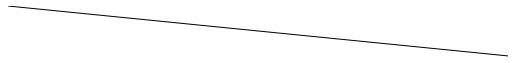
\includegraphics[width=\textwidth]{img/line.png}
\end{frame}

\subsection{Axes}

\begin{frame}
  \frametitle{Axes}
  D3 Axes are functions whose parameters we define. When called, it generates the visual elements of the axis, including lines, labels and ticks. 
  \newline

  Axes are SVG-specific, as they generate SVG elements. They must be applied to either SVG or SVG \textbf{group} elements. 
\end{frame}

\begin{frame}
  \frametitle{SVG Groups}
  The \textbf{g} element within SVG stands for the \textit{group} element. Group elements are invisible, but they allow us to:
  \begin{itemize}
  \item<1-> Contain / \textbf{group} elements together
  \item<2-> We can apply transformations to these groups
  \end{itemize}
\end{frame}

\begin{frame}
  \frametitle{Constructing an axis function}
  \lstaxis
\end{frame}


\begin{frame}
  \frametitle{Usage}
  \lstcreateaxis
\end{frame}

\subsection{SVG Paths}
\begin{frame}
  An SVG path can draw all sorts of shapes - rectangles, circles, ellipses, straight lines, curves and polygons. 
  \newline

  The shape of an SVG Path element is defined by the attribute \textit{\textbf{d}}, which contains the series of commands and parameters from within the SVG Path Mini-Language. 
  \newline

  These commands are analogous to a set of instructions for \textit{how to move a pen on paper}.
\end{frame}

\begin{frame}
  \lstsvgtriangle
\end{frame}

\begin{frame}
  \begin{itemize}
  \item<1->M 10 25: Put the pen down at (10, 25)
  \item<2->L 10 75: Draw a line to the point (10, 75) from (10, 25)
  \item<3->L 60 75: Draw a line to the point (60, 75) from (10, 75)
  \item<4->L 10 25: Draw a line to the point (10, 25) from (60, 75)
  \end{itemize}

  Note that SVG Path commands are case sensitive. \textbf{Capitalcase} means we are using \textit{absolute positioning} based on the
  SVG viewing window, \textbf{lowercase} means we are using \textit{relative positioning}. 
\end{frame}

\subsection{D3 Selection Pattern}
\begin{frame}
  \frametitle{Update}
  selection.\textbf{data()}: Joins an array of data to the current selection. Results in the \textit{update} selection, which represents the selected DOM elements that were successfully bound to the specified data elements.
  \newline

  The \textit{update} method also contains a reference to the \textit{enter} and \textit{exit} selection, used for adding and removing nodes in correspondence with the data.
\end{frame}

\begin{frame}
  \frametitle{Enter}
  selection.\textbf{enter()}: Returns the enter selection - placeholder nodes for each data for which no corresponding existing DOM element was found. Supports the following operators:
  \begin{itemize}
  \item<1->append
  \item<2->insert
  \item<3->select
  \item<4->call
  \end{itemize}

\end{frame}

\begin{frame}
  \frametitle{Exit}
  selection.\textbf{exit()}: Contains existing DOM elements in the current selection for which no data element was found. Exposes the \textbf{remove} operator, which allows the removal of these elements. 
\end{frame}

\begin{frame}
  \frametitle{Example}
  \lstexit
\end{frame}

\begin{frame}
  \frametitle{Example}
  \lstexitl
\end{frame}

\subsection{JavaScript callbacks}
\begin{frame}
  \frametitle{Why callbacks?}
  Callbacks in JavaScript are a pattern which solve the problem of dealing with its asynchronous behavior. Functions in JavaScript are first-class objects, meaning that they can be passed around as arguments to other functions. 

  \lstcallback
\end{frame}

\subsection{Resources}
\begin{frame}
  \frametitle{D3 Resources}
  \begin{itemize}
  \item<1-> Tutorials: https://github.com/mbostock/d3/wiki/Tutorials
  \item<2-> API: https://github.com/mbostock/d3/wiki/API-Reference
  \item<3-> Stackoverflow
  \end{itemize}
\end{frame}


\end{document}
